\documentclass[../main.tex]{subfiles}
\graphicspath{{\subfix{../../img/}}}
\begin{document}

\newpage
\section{Konzeptfindung}
\label{a3:Konzeptfindung}

Das Projektteam hat sich als Ziel gesetzt, ein möglichst einfaches und zuverlässiges Gesamtkonzept zu finden, welches robust ist und fehlerunanfällig funktioniert. Dies wird erreicht, in dem vorgängig alle Lösungsansätze aus der Technologierecherche, die mit grossen Risiken verbunden sind, erkannt und herausgefiltert werden. Mit den verbleibenden Ansätzen wird ein Morphologischer Kasten erstellt, um das Gesamtkonzept zu entwickeln. Damit mit dem Morphologischen Kasten die optimale Variante gefunden werden kann, wird zu einigen Teilfunktionen des Fahrzeuges eine Nutzwertanalyse erstellt.

\subsection{Vorauswahl}
\label{a3:Vorauswahl}
    \subsubsection{Fortbewegung}
    Das Fahrzeug muss in der Lage sein, sich an Ort und Stelle um die eigene Achse zu drehen. Somit sind die Optionen Knicklenkung, Achsschenkellenkung und Drehschemellenkung nicht geeignet.
    Das Prinzip ''Fahrzeug abbocken und drehen'' ist als alleiniges Lenksystem ungeeignet, weil es zu viel Zeit benötigt für das Lenkmanöver. 
    Omniwheels und Mecanum-Räder sind sehr ähnlich, nur die Form und Anordnung der Rollen auf den Rädern ist unterschiedlich. Bei Omniwheels sind die Rollen in einem Winkel von 90° an den Rädern befestigt, wobei sie bei Mecanum-Rädern in 45° angeordnet sind und eine Tonnenform aufweisen. Dadurch versprechen die Mecanum-Räder eine geringere Anfälligkeit, sich in den Plattenfugen zu verfangen. Die 4-Rad Differenzial Lenkung und das Prinzip Roomba sind von der Wendigkeit und dem konstruktiven Aufwand vergleichbar, jedoch besteht bei der 4-Rad Variante die Gefahr von Aufschaukeln bei einer Drehung an Ort und Stelle, sowie die Gefahr von Schieben der langsameren Räder bei Kurvenfahrt. Mit diesen Erkenntnissen kommen nur noch die Mecanum-Räder und das Prinzip Roomba in Frage. Die beiden Systeme werden in einer Nutzwertanalyse (Tabelle \ref{tab:nutzwertanalyse_fortbewegung}) genauer verglichen und bewertet.
        
\newpage
\subsubsection{Hindernis Bewältigung}
    \paragraph{Aufnahme}
    Weil das Konzept möglichst einfach und zuverlässig gestaltet werden soll, scheiden die Ideen ''Gabelstapler'' und ''Vakuum-Sauggreifer'' aus. Der Gabelstapler erfordert eine äusserst präzise und aufwendige Sensorik, um die Löcher für die Aufnahme genau zu treffen. Der ''Vakuum-Sauggreifer'' weist im Vergleich zu den ''Klemmen'' eine geringere technische Zuverlässigkeit auf. Da wir keine Erfahrung mit dieser Technologie haben, wären umfangreiche Tests notwendig, um eine vergleichbare Sicherheit zu erreichen. Zudem bietet der ''Vakuum-Sauggreifer'' keine wesentlichen Vorteile gegenüber den ''Klemmen''.

        
    \paragraph{Rotation und Translation}
    Ein beweglicher Arm erhöht die Komplexität sowohl mechanisch als auch in den Bereichen Sensorik und Software erheblich. Dabei ist zu beachten, dass die Integration eines Arms die Gesamtkomplexität steigert, ohne in anderen Bereichen nennenswerte Vereinfachungen zu ermöglichen. Dies widerspricht unserem Grundprinzip, eine möglichst einfache und zuverlässige Lösung zu entwickeln. Daher werden alle Optionen mit einem beweglichen Arm ausgeschlossen, sodass lediglich die Option ''Rotation des Fahrzeugs'' verbleibt.


\newpage
\subsubsection{Wegfindung}

Der zu befahrende Graph ist bereits vorgegeben. Er hat acht Knoten und 15 Kanten, was 
für einen Algorithmus relativ klein ist. Die Effizienz und Dynamik des Algorithmus spielt keine grosse Rolle, weil der Zeitunterschied der Algorithmen bei einer Neuberechnung nur minimal ist. Dafür werden Kriterien wie geringer Speicherbedarf und niedrige Komplexität höher gewertet. Ausgeschlossen wurden folgende Algorithmen: Der Algorithmus ''Goal directed shortest path queries using precomputed cluster distances'' wird aufgrund der hohen Komplexität und des hohen Speicherbedarfs nicht weiter analysiert. Der Floyd Warshall-Algorithmus, der sich auf die Berechnung aller kürzesten Pfade in einem Graphen fokussiert, entspricht nicht unserem Anwendungsbereich und wird ebenfalls nicht weiter betrachtet.


\subsubsection{Objekterkennung}

Bei der Objekterkennung sind die Schnelligkeit und der Ressourcenbedarf sehr wichtige Kriterien.
Da die Erkennung auf einem Raspberry Pi läuft und so viele Bilder pro Sekunde wie möglich analysieren soll, muss sie möglichst schnell und ressourceneffizient sein. 

R-CNN ist von den vier recherchierten Objekterkennungsmethoden die Langsamste und Ressourcen intensivste, weshalb sie bereits in der Vorauswahl ausscheidet.


\subsection{Morphologischer Kasten}\label{morphologischer kasten}

    \imageheight{assets/MorphologischerKasten.pdf}{Morphologischer Kasten}{0.88\textheight}
    

    \subsubsection{Variantenbeschreibung}
    Folgend werden die verschiedenen Lösungskonzepte kurz beschrieben und nachfolgend die einzelnen Optionen diskutiert und bewertet.
    \paragraph{Lösungsvariante Simpel (grün)} 
    \label{a3:loesungsvariante_Simpel}
    Bei der Lösungsvariante ''Simpel'' liegt der Schwerpunkt auf der Einfachheit und Zuverlässigkeit des Konzepts. Die Fortbewegung und Lenkung erfolgen nach dem ''Roomba''-Prinzip, bei dem zwei Räder jeweils von einem DC-Motor angetrieben werden. Dieses Konzept ermöglicht eine einfache Steuerung und eine Drehung auf der Stelle.

    Hindernisse werden seitlich geklemmt und aufgenommen, wobei der Antrieb dafür durch einen DC-Motor realisiert wird. Dieser besizt zwei Mikroschalter als Endanschläge. Nachdem Aufnehmen des Hindernisses dreht sich das Fahrzeug um die eigene Achse und setzt es anschliessend wieder ab. Zur Überprüfung der Position der DC-Motoren werden Encoder verwendet. Diese sind aufgrund ihrer einfachen Funktionsweise und ihrer zuverlässigen Ausgabe besonders geeignet.

    Die Software läuft auf einem Raspberry Pi, während die Hardwaresteuerung durch einen TinyK22 erfolgt. Das Projektteam besitzt bereits Knowhow für beide dieser Plattformen. Die Hinderniserkennung für die Aufnahme wird mithilfe eines Ultraschallsensor durchgeführt. Dieser hat sich für den Anwendungsfall behauptet (siehe \ref{sec:Distanz_Hindernis}). 

    Pylonen und Hindernisse auf dem Weg werden mithilfe einer Kamera erkannt. Für die Erkennung des nächsten Zielpunkts wird dieselbe Kamera verwendet. Ein Liniensensor stellt sicher, dass sich das Fahrzeug korrekt entlang des Klebestreifens bewegt. Der Liniensensor ist dabei die einfachste Lösung zur Linienerkennung. Ähnlich verhält es sich bei der Verifizierung von Wegpunkten, die ebenfalls primär durch den Liniensensor erkannt werden. Dabei wird festgestellt, dass ein Wegpunkt vorliegt, wenn die Linie eine bestimmte Dicke überschreitet. 

    Die Software für die Objekterkennung basiert auf YOLO, während für die Wegfindung der Dijkstra-Algorithmus eingesetzt wird. Die Energieversorgung erfolgt durch einen Lithium-Polymer-Akku, aufgrund seiner zahlreichen Vorteile (siehe \ref{a3:Energiequelle}).
    
    \newpage
    
    \paragraph{Lösungsvariante Beweglich (gelb)}
    \label{a3:loesungsvariante_beweglich}
    Bei der Lösungsvariante ''Beweglich'' liegt der Fokus auf der Beweglichkeit des Fahrzeugs. Die Fortbewegung und Lenkung erfolgen mit Mecanum-Rädern, wobei jedes der vier Räder von einem Schrittmotor angetrieben wird. Dadurch kann sich das Fahrzeug in alle vier Richtungen linear bewegen, was ermöglicht, das Fahrzeug präzise auf ein Hindernis auszurichten.

    Das Hindernis wird von vorne und hinten geklemmt und aufgenommen, wobei der Antrieb durch einen Schrittmotor erfolgt, der eine exakte Klemmung ermöglicht. Nachdem das Hindernis aufgenommen wurde, dreht sich das Fahrzeug um die eigene Achse und setzt es wieder ab. Die Position des Fahrzeugs wird mithilfe eines Beschleunigungssensors überwacht. Dies ermöglicht eine präzise Erfassung der Fahrzeugbewegung, obwohl sich das Fahrzeug in alle Richtungen bewegen kann. Zudem werden Schrittfehler der Schrittmotoren abgefangen.

    Die Software läuft auf einem Raspberry Pi, während die Hardwaresteuerung durch einen Arduino erfolgt. Der Vorteil des Arduinos liegt in der grossen Community und der Vielzahl an Hilfestellungen, die im Internet verfügbar sind.

    Die Hindernisse werden mit einem Infrarotsensor erkannt. Zur Sicherstellung der Redundanz wird ein Ultraschallsensor eingesetzt, um zu überprüfen, ob tatsächlich ein Hindernis im Weg steht.

    Die Fahrstrecke wird hauptsächlich mit einem Liniensensor erfasst. Die Kamera gibt an, in welchem Winkel der nächste Wegpunkt liegt. Wegpunkte werden durch den Liniensensoren erkannt und mit einem Farbsensor bestätigt. Die Software für die Objekterkennung basiert auf YOLO, während die Wegfindung den A*-Algorithmus nutzt.

    Für die Energieversorgung wird ein Lithium-Ionen-Akku eingesetzt, da hierfür auch eine handelsübliche Powerbank verwendet werden könnte.

    \paragraph{Entscheid Lösungsvariante}
    \label{a3:EntscheidLösungsvariante}
    Umgesetzt wird die Lösungsvariante ''Simpel'' (grün), aufgrund ihrer Einfachheit und Robustheit. Bei der Lösungsvariante ''Beweglichkeit'' (gelb) bestehen zu viele Risiken. Zum Beispiel ist die Ansteuerung der Schrittmotoren mit den Mecanum-Rädern wesentlich komplexer als beim Roomba-Prinzip. Ausserdem reicht für die ''Simpel''-Lösungsvariante die Toleranz von etwa 2 cm beim Zurückstellen des Hindernisses aus. Bei der ''Beweglichkeit''-Lösungsvariante wäre das Hindernis zwar präziser zurückgestellt, jedoch mit vielen Unsicherheiten verbunden.

    Zudem wird der TinyK22 bevorzugt, da die Elektrotechniker bisher keine Erfahrung mit Arduinos haben und der TinyK22 bereits intensiv im Unterricht behandelt wurde. Das Ziel der Gruppe ist es, das Ziel sicher zu erreichen, und dafür eignet sich die ''Simpel''-Lösungsvariante am besten.
    
    \subsubsection{Fortbewegung}
    \label{a3:Fortbewegung}
    Damit eine genauere Analyse zwischen Mecanum-Rädern und dem Prinzip Roomba durchgeführt werden kann, wird eine Nutzwertanalyse erstellt. Der Gewinner ist das Prinzip Roomba (ersichtlich in Tabelle \ref{tab:nutzwertanalyse_fortbewegung}).

    \begin{table}[H]
        \textbf{Legende:}
        \hspace{1cm}
        \textbf{GW:} Gewichtung
        \hspace{1cm}
        \textbf{BW:} Bewertung
        \hspace{1cm}
        \textbf{PT:} Punkte
        \vskip 3 mm
        \resizebox{\textwidth}{!}{
        \centering
        \renewcommand{\arraystretch}{1.5}
        \scriptsize
        \begin{tabular}[H]{|p{2cm}|p{3cm}|c|c|c|p{2.5cm}|c|c|p{2.5cm}|}
            \hline
            \multicolumn{3}{|c|}{} & 
            \multicolumn{3}{c|}
            {\textbf{Mecanum-Rad}} & 
            \multicolumn{3}{c|}{\textbf{Prinzip Roomba}}\\ \hline
             \textbf{} & \textbf{Erklärung} & \textbf{GW} & \textbf{BW} & \textbf{PT} & \textbf{Begründung} & \textbf{BW} & \textbf{PT} & \textbf{Begründung} \\ 
            \hline
            Manövrierbarkeit & Wie einfach kann in alle Richtungen manövriert werden & 30 & 9 & 270 & Ist in alle Richtungen beweglich ohne vorgängige Drehung & 6 & 180 & Muss drehen, um in eine andere Richtung zu fahren \\
            \hline
            Resistenz gegen Verfangen in Plattenfugen & Wie anfällig sind die Räder auf Verfangen in den Plattenfugen und damit verbundene Fahrfehler & 35 & 5 & 175 & Kleine Rollen am Radumfang, welche in Fugen passen & 8 & 280 & Nur kleines Stützrad, welches in Fugen passt, Stützrad ist passiv für die Lenkung \\
            \hline
            Komplexität & Wie aufwendig ist die Konstruktion und Programmierung & 20 & 4 & 80 & 4 Motoren ansteuern und hoher Rechenaufwand & 8 & 160 & Nur 2 Motoren nötig \\
            \hline
            Kosten & Wie viel kostet die Vorrichtung & 15 & 4 & 60 & 4 Motoren nötig & 8 & 120 & Nur 2 Motoren nötig \\
            \hline
             Nutzwert & \textbf{Gesamtnutzwert} & 100 & & 585 & & & 740 & \\
            \hline
        \end{tabular}
        \normalsize
        }
        \caption{Nutzwertanalyse Fortbewegung}
        \label{tab:nutzwertanalyse_fortbewegung}
    \end{table}

Das Prinzip Roomba ist von allen recherchierten Fortbewegungssystemen (siehe Anhang \ref{recherche-prinzip-roomba}) dasjenige, welches mit den wenigsten Komponenten auskommt und den geringsten Programmieraufwand benötigt. Dadurch verspricht es robust und am wenigsten fehleranfällig zu sein. Als Stützelement wird nicht wie üblich ein drehbares Rad verwendet, sondern ein Gleitelement. Der Grund dafür ist die Gefahr, dass bei einem Rad ein Versatz entsteht, wenn es sich neu ausrichten muss. Das Problem kann man sich wie bei einem Einkaufswagen vorstellen: Wenn man damit wenden will, fährt der Einkaufswagen bekanntlich immer einen kleinen Schwenker, bevor die Räder wieder in die gewünschte Richtung zeigen.

Eine andere Möglichkeit wäre eine Kugel, jedoch hat ein etwas grossflächigeres Gleitelement den Vorteil, dass es weniger in die Plattenfugen rutscht. Das Gleitelement wird im hinteren Teil des Fahrzeuges angebracht, weil vorne aufgrund des Mechanismus zur Hindernisaufnahme kein Platz dafür besteht. Bei dieser Anordnung muss darauf geachtet werden, dass der Schwerpunkt des Fahrzeuges auch mit aufgenommenem Hindernis hinter der Kippachse (Achse der Antriebsräder) liegt. Dies wird mit der Anordnung des Akkus im hintersten Teil des Fahrzeuges sichergestellt.

Das Risiko R15 ''Verschieben bei Drehung'' (siehe Kapitel \ref{risikomatrix}) könnte mitigiert werden,
indem optional eine zusätzliche Funktion für das Drehen des Fahrzeugs eingebaut werden kann, falls das Risiko eintreten sollte.

Bei dieser Ersatz-Rotation würde das Fahrzeug aufgebockt werden um sich zu drehen.
Diese Methode ist zwar viel langsamer, würde jedoch sicherstellen, dass sich das Fahrzeug 
beim Drehen nicht verschiebt. Der Aufwand für eines zusätzlichen Drehmechanismus wurde allerdings zu einem späteren Zeitpunkt im Projekt verworfen, da er gegen das Simpel-Prinzip verstösst und sehr aufwändig wäre. Das Risiko wird akzeptiert.

\subsubsection{Fahrantrieb}
\label{a3:Fahrantrieb}
Bei der Auslegung des Antriebs ergaben sich drei Varianten. Der Schrittmotor, DC-Motor und der Brushlessmotor. Da die Ansteuerung möglichst einfach gehalten werden soll, ist der Brushlessmotor mit seiner komplexeren Ansteuerung ungeeignet. Der Vorteil des Schrittmotors ist, dass dieser nicht unbedingt auf einen Encoder oder ähnliches angewiesen ist. Dieser kann man genau schrittweise ansteuern und somit seine Position verfolgen. Der Nachteil ist, dass es ein Open-Loop Regelung wäre, also ohne Rückführgrösse. Dies bedeutet, dass der Schrittmotor bei einer mechanischen Überlastung Schritte zurückmelden würde, die er in Realität nicht gefahren ist. Auch dieser Motor hat eine schwierigere Ansteuerung mithilfe von Drivers. Ausserdem sind Schrittmotoren relativ schwer. Der DC-Motor ist dagegen der einfachste zum Ansteuern. Dieser benötigt eine einen einfachen Motortreiber (H-Brücke), der einfach anzusteuern ist. Ausserdem kann man hohe Drehmomente mittels Übersetzungen erreichen. Das macht den DC-Motor zum bevorzugten Antriebsmotor für die Fahrt. Bei genügend grosser Auslegung, würde sich der Schrittmotor ebenso eignen. 

\subsubsection{Hindernisbewältigungsantrieb}
\label{a3:Hindernisbewältigungsantrieb}
Für die Hindernisbewältigung wird ebenfalls ein Antrieb benötigt. Dafür wird ein DC-Motor verwendet. Dieser braucht keine komplexe Ansteuerung, da der DC-Motor nur Ein- und Ausgeschaltet wird, ohne Geschwindigkeitsregelung. Der DC-Motor muss nur in die zwei Endschalter geklemmt oder gelöst fahren. Der Schrittmotor könnte theoretisch ohne Endschalter auskommen, indem vorher die benötigte Anzahl an Schritten ermittelt werden und dann je nach klemen oder lösen diese Anzahl Schritt gefahren werde. Dies birgt natürlich das Risiko von möglichen Schrittverlusten mit der Zeit.

  
\subsubsection{Sensorik Positionsabfrage}
\label{a3:Sensorik:Positionsabfrage}
Zur Auswahl stehen ein Encoder und ein Beschleunigungssensor. Der Encoder liefert auf Dauer genauere Daten und der Aufbau ist einfacher. Beim Beschleunigungssensor nimmt der Messfehler mit der Zeit zu und muss andauernd wieder kalibriert werden. Es wäre möglich, die Sensoren an jedem Wegpunkt zu kalibrieren, um Messfehler zu korrigieren. Der Encoder spielt eine entscheidende Rolle, da er sicherstellt, dass die Motoren die gleiche Anzahl an Umdrehungen ausführen. Dies ist insbesondere bei Drehbewegungen von großer Bedeutung, da andernfalls falsche Winkel erreicht werden könnten.

\subsubsection{Software Steuerung}
Bei der Softwaresteuerung kommt wegen der Grösse und Leistung nur das Raspberry Pi in Frage.
Eine Alternative wäre noch ein Arduino, jedoch reicht dies für leistungsintensive Aufgabe wie
Objekterkennung nicht aus.

\newpage

\subsubsection{Hardware Steuerung}
\label{a3:Hardware Steuerung}
Damit man die Aktoren und Sensoren auswerten kann, benötigt es eine hardwarenahe Steuerung, die mit dem Raspberry Pi kommuniziert. Aus der Recherche ergaben sich dafür drei Möglichkeiten. Ein Arduino, TinyK22 oder ein ESP32. Dabei scheidet der ESP32 vor allem durch seine nicht benötigten Funktionen aus. Weder Wifi noch Bluetooth werden benötigt. Damit bleiben noch der TinyK22 und ein Arduino-Board. Aufgrund Ihrer Ähnlichkeit wurde eine Nutzwertanalyse erstellt (siehe Tabelle \ref{tab:konzept_nutzwertanalyse_mikrocontroller}).

    \begin{table}[H]
        \textbf{Legende:}
        \hspace{1cm}
        \textbf{GW:} Gewichtung
        \hspace{1cm}
        \textbf{BW:} Bewertung
        \hspace{1cm}
        \textbf{PT:} Punkte
        \vskip 3 mm
        \resizebox{\textwidth}{!}{
         \centering
         \renewcommand{\arraystretch}{1.5}
             \begin{tabular}{|p{2.5cm}|>{\raggedright} p{3cm}|c|c|c|>{\raggedright} p{3cm}|c|c|>{\raggedright\arraybackslash}p{3cm}|}
                \hline
                \multicolumn{3}{|c|}{} & \multicolumn{3}{c|}{\textbf{Arduino}} & \multicolumn{3}{c|}{\textbf{TinyK22}} \\ \hline
                \textbf{Kriterium} & \textbf{Erklärung} & \textbf{GW} & 
                \textbf{BW} & \textbf{PT} & 
                \textbf{Begründung} & \textbf{BW} & 
                \textbf{PT} & \textbf{Begründung} \\ \hline

                Libraries & Sind Frameworks vorhanden & 20 & 9 & 180 & Grosse Anzahl Online Libraries & 8 & 160 & McFun Bibliothek \\ \hline
                Online Informationen & verfügbare Skripte / Beschriebe vorhanden? & 30 & 8 & 240 & Viele Online Tutorials & 6 & 180 & Blog von M. Styger und McFun Folien \\ \hline
                I/O Pins & Anzahl frei verfügbare GPIO & 30 & 6 & 180 & 22 Pins beim nano & 8 & 240 & 28 Pins verfügbar \\ \hline
                Finanziell & Wie viel kostet der Mikrocontroller & 10 & 6 & 60 & Um die 20CHF & 9 & 90 & Evtl. von der Schule \\ \hline
                Nachhaltigkeit & Energieverbrauch für die Beschaffung & 10 & 7 & 70 & Arduino bereits von Privatgebrauch vorhanden & 9 & 90 & Bereits vorhanden aus früheren Modulen \\ \hline
                \multicolumn{2}{|r|}{\textbf{Nutzwert:}} & 100 & & 730 & & & 760 & \\ \hline
            \end{tabular}
         }
            \caption{Nutzwertanalyse der Mikrocontroller}
            \label{tab:konzept_nutzwertanalyse_mikrocontroller}
        \end{table}

    Der Vorteil des Arduinos liegt in seiner grossen Community und der umfangreichen Online-Hilfe, die zur Verfügung steht. Da jedoch die Elektrotechniker keine Programmiererfahrung in C++ haben und nicht jeder Arduino eine Debugging-Funktion bietet, ist der Arduino nicht die geeignete Lösung.

    Der TinyK22 hingegen wurde im Modul Mc Fun ausführlich behandelt. Er bietet eine benutzerfreundliche Programmierumgebung mit integriertem Debugger und wird in C programmiert. Zudem können bei Fragen die Dozenten konsultiert werden, die bereits über umfangreiche Erfahrung mit dem TinyK22 verfügen. In unserem Anwendungsfall stellt der TinyK22 daher die einfachste und effektivste Lösung für die Programmierung dar.


\subsubsection{Objekterkennung Sensor}
\label{a3:Objekterkennung_Sensor}
Wie in Kapitel \ref{sec:Distanz_Hindernis} beschrieben, zeigte der Test der Sensorik, dass der Ultraschallsensor ab einer minimalen Distanz von 3 cm zuverlässige Messwerte liefert. Er ist ebenso unabhängig der Sonnenlichteinstrahlung. Der Infrarotsensor reagiert stärker auf Sonnenlichteinstrahlung und misst ungefähr die gleichen Werte. 



\subsubsection{Streckenerkennung}
Für die Streckenerkennung soll eine Kamera verwendet werden. Die Kamera erkennt Hindernisse und Pylonen auf der Strecke und hilft dem Raspberry Pi so die beste Strecke zu ermitteln. Damit das Fahrzeug auf der Linie bleibt, wird ein Liniensensor eingesetzt.  Im Kapitel \ref{sec:Linienerkennung_Punkterkennung_Test} wurden ebenfalls der \gls{ir-fototransistor} vermessen, welcher für den Liniensensor eingesetzt wird. Diese Messungen ergaben, dass sich die Aufladezeit des Kondensators gegenüber der verschiedenen Untergründe stark unterscheiden. Für weitere Details siehe Kapitel \ref{sec:Linienerkennung_Punkterkennung_Test}. 

\subsubsection{Punktverifizierung}
Um zu erkennen, ob das Fahrzeug sich auf einem Punkt befindet, könnte ein Farbsensor genutzt werden. Dieser gibt die drei Primärfarben in je einem Digitalsignal zurück. Dieser scheidet aufgrund von Tests aus (siehe Kapitel \ref{sec:Linienerkennung_Punkterkennung_Test}) aus. Die Variante mit der Kamera wird ausgeschlossen, da der Einsatz von zwei Kameras das Budget erheblich überschreiten würde. Eine einzelne Kamera beansprucht bereits 1/5 des verfügbaren Budgets, und für die Anwendung wären zwei Kameras erforderlich. Eine Kamera müsste in einer bestimmten Höhe für die Strecken- und Objekterkennung positioniert werden, während die andere Kamera möglichst nah an der Linie für die Linienerkennung platziert werden müsste.

Ein Liniensensor bietet hingegen eine kostengünstigere Lösung. Er könnte so dimensioniert werden, dass er den Punkt anhand des Durchmessers erkennt. Wenn der Liniensensor direkt über dem Punkt positioniert ist, würden alle IR-Fototransistoren die Linie erkennen, was auf das Vorhandensein eines Punktes hinweist.

\newpage

\subsubsection{Objekterkennung Software}
\label{a3:Objekterkennung}
Bei der Technologierecherche wurden vier verschiedene Objekterkennungsmethoden recherchiert, wobei R-CNN bereits in der Vorauswahl ausschied, weil sie langsam und ressourcenintensiv ist.
Dieser Abschnitt fokussiert sich darauf, anhand von einer Nutzwertanalyse von den restlichen drei Auswahlen die Beste zu treffen.

Für die Nutzwertanalyse werden die folgenden Kriterien verwendet.

\begin{itemize}
\item \textbf{Genauigkeit}: Das wichtigste Kriterium ist, dass alle Objekte, die in einem Bild ersichtlich sind, genau erkannt werden.
\item \textbf{Geschwindigkeit}: Die Bilder werden während des Fahrens analysiert. Eine schnelle Objekterkennungsmethode ist essenziell, damit das Fahrzeug schnell reagieren kann.
\item \textbf{Ressourcenbedarf}: Die Objekterkennung erfolgt on-board auf ressourcenlimitierter Hardware. Somit soll die Erkennung möglichst effizient sein.
\item \textbf{Komplexität}: Das Projekt ist zeitlich limitiert. Der Aufwand für die Implementierung der Objekterkennung berücksichtigt werden. Dazu gehört auch die Menge der benötigten Trainingsdaten.
\end{itemize}

\begin{table}[H]
\resizebox{\textwidth}{!}{
 \centering
 \renewcommand{\arraystretch}{1.5}
     \begin{tabular}{|c|c|c|c|c|c|c|c|}
        \hline
        \multicolumn{2}{|c|}{} & 
        \multicolumn{2}{c|}{\textbf{CNN}} &
        \multicolumn{2}{c|}{\textbf{YOLO}} &
        \multicolumn{2}{c|}{\textbf{Haar-Cascade}} \\
        \hline
        
        \textbf{Kriterium} & \textbf{Gewicht} &
        \textbf{Bewertung} & \textbf{Punkte} &
        \textbf{Bewertung} & \textbf{Punkte} &
        \textbf{Bewertung} & \textbf{Punkte} \\
        \hline

        Genauigkeit & 40 &
        8 & 320 &
        7 & 280 &
        5 & 200 \\
        \hline

        Geschwindigkeit & 30 &
        6 & 180 &
        9 & 270 &
        8 & 240 \\
        \hline

        Ressourcenbedarf & 20 &
        4 & 80 &
        6 & 120 &
        8 & 160 \\
        \hline

        Komplexität & 10 &
        2 & 20 &
        5 & 50 &
        7 & 70 \\
        \hline
        
        \textbf{Nutzwert:} & 100 & & 590 & & 720 & & 670 \\ \hline
    \end{tabular}
 }
    \caption{Nutzwertanalyse Objekterkennung}
    \label{tab:nutzwertanalyse_objekterkennung}
\end{table}

YOLO erreicht in der durchgeführten Nutzwertanalyse (siehe Tabelle \ref{tab:nutzwertanalyse_objekterkennung}) die beste Gesamtbewertung. Es erlaubt eine effiziente und relativ genaue Analyse der Bilder.
Haar-Cascade ist ebenfalls schnell und ressourcenschonend, schneidet aber in der wichtigsten Kategorie ''Genauigkeit'' schlecht ab.
CNN, das in der Kategorie Genauigkeit die beste Bewertung erzielte, zeigt deutliche Schwächen in Bezug auf ''Geschwindigkeit'', ''Ressourcenbedarf'' und ''Komplexität''.

\newpage

\subsubsection{Wegfindung}
\label{a3:Wegfindung}
Der geeignetste Wegfindungsalgorithmus wird anhand einer Nutzwertanalyse mit den folgenden Kriterien gefunden.

\begin{itemize}
    \item \textbf{Einfachheit:} Einfach zu implementieren oder bereits in bekannten Bibliotheken vorhanden.
    \item \textbf{Genauigkeit:} Findet \textbf{garantiert} den kürzesten Weg.
    \item \textbf{Dynamisch:} Kann sich dynamisch auf Graphveränderungen anpassen.
    \item \textbf{Schnelligkeit:} Wie schnell der kürzeste Weg berechnet werden kann.
    \item \textbf{Effizienz:} Benötigter Leistungs- und Speicheraufwand
\end{itemize}

\begin{table}[H]
\resizebox{\textwidth}{!}{
 \centering
 \renewcommand{\arraystretch}{1.5}
     \begin{tabular}{|c|c|c|c|c|c|c|c|c|c|}
        \hline
        \multicolumn{2}{|c|}{} & 
        \multicolumn{2}{c|}{\textbf{Dijkstra}} &
        \multicolumn{2}{c|}{\textbf{A*}} &
        \multicolumn{2}{c|}{\textbf{D*}} &
        \multicolumn{2}{c|}{\textbf{RRT}} \\ 
        \hline
        
        \textbf{Kriterium} & \textbf{Gewicht} &
        \textbf{Bewertung} & \textbf{Punkte} &
        \textbf{Bewertung} & \textbf{Punkte} &
        \textbf{Bewertung} & \textbf{Punkte} &
        \textbf{Bewertung} & \textbf{Punkte} \\
        \hline

        Einfachheit & 10 &
        10 & 100 &
        7 & 70 &
        5 & 50 &
        3 & 30 \\
        \hline

        Genauigkeit & 60 &
        10 & 600 &
        8 & 480 &
        8 & 480 &
        6 & 360 \\
        \hline

        Dynamisch & 5 &
        1 & 5 &
        1 & 5 &
        10 & 50 &
        5 & 25 \\
        \hline

        Schnelligkeit & 5 &
        7 & 35 &
        8 & 40 &
        9 & 45 &
        5 & 25 \\
        \hline

        Effizienz & 20 &
        9 & 180 &
        7 & 140 &
        4 & 80 &
        2 & 40 \\
        \hline
        
        \textbf{Nutzwert:} & 100 & & 920 & & 735 & & 705 && 480 \\ \hline
    \end{tabular}
 }
    \caption{Nutzwertanalyse Wegfindung}
    \label{tab:nutzwertanalyse_wegfindung}
\end{table}

Die Nutzwertanalyse zeigt Dijkstra als deutlichen Gewinner. Dies liegt vor allem an der hohen Genauigkeit, Einfachheit und Effizient. Einzig bei der nicht vorhandenen Dynamik schneidet Dijkstra schlecht ab. Aufgrund des kleinen Graphen spielt das jedoch keine grosse Rolle, da der Weg einfach neu berechnet werden kann.

\newpage

\subsubsection{Energiequelle}
\label{a3:Energiequelle}
Zur Auswahl stehen Li-Po, Li-Ion oder NiMh Akkus. Der Li-Po und Li-Ion Akku haben die höhere Energiedichte als der NiMh Akku. Jedoch benötigt der Li-Po Akku einen Laderegler für die Aufladung und der Li-Ionen Akku benötigt eine elektrische Schutzschaltung. Zwischen dem Li-Ion und dem Li-Po Akku gibt es keine weiteren nennenswerten Unterschiede. 
Im Vergleich zu dem NiMh Akku benötigen sie weniger Platz und sind leichter. Ebenso haben sie keinen Memoryeffekt und eine geringere Selbstentladung als der NiMh Akku. Die Lebensdauer eines NiMh Akkus ist dagegen fast fünfmal so lange wie die eines Lipo-Akkus \cite{nimh_vs_lipo_rcteam}. Für den Entscheid wurde eine Nutzwertanalyse erstellt:


\begin{table}[H]
        \resizebox{\textwidth}{!}{
         \centering
         \renewcommand{\arraystretch}{1.5}
             \begin{tabular}{|c|>{\raggedright} p{3cm}|c|c|c|>{\raggedright} p{3cm}|c|c|>{\raggedright\arraybackslash}p{3cm}|}
                \hline
                \multicolumn{3}{|c|}{} & \multicolumn{3}{c|}{\textbf{LiPo}} & \multicolumn{3}{c|}{\textbf{NiMh}} \\ \hline
                \textbf{Kriterium} & \textbf{Erklärung} & \textbf{Gewichtung} & \textbf{Bewertung} & \textbf{Punkte} & \textbf{Begründung} & \textbf{Bewertung} & \textbf{Punkte} & \textbf{Begründung} \\ \hline
                Lebensdauer & Wie lange hält der Akku & 10 & 6 & 60 & Bis 200 Ladezyklen & 8 & 80 & Bis 1000 Ladezyklen \\ \hline
                Leistungsdichte & Energie / Volumen & 30 & 9 & 270 & Hohe Energiedichte & 6 & 180 & Mittlere Energiedichte \\ \hline
                Leistungsabgabe & Wie viel Strom kann gezogen werden & 30 & 8 & 240 & Hohe Entladungsrate  & 4 & 120 & Niedrige Entladungsrate \\ \hline
                Sicherheit & Brenngefahr & 20 & 4 & 80 & Gefahr bei unsachmässigem Gebrauch & 8 & 160 & Keine Gefahr \\ \hline
                Kosten & Wie viel kostet der Akku & 10 & 4 & 40 & Um die 30CHF & 7 & 70 & Um die 20CHF \\ \hline
                \multicolumn{2}{|r|}{\textbf{Nutzwert:}} & 100 & & 690 & & & 610 & \\ \hline
            \end{tabular}
}
            \caption{Nutzwertanalyse Akku}
            \label{tab:konzept_Akku}
        \end{table}
        

Aus der Nutzwertanalyse geht hervor, dass der Li-Po Akku verwendet wird. Diese Akkus werden hauptsächlich für den Modellbau verwendet. Wie gemacht für einen Prototyp. Der NiMh Akku wird nicht verwendet, da dieser eine geringe Leistungsabgabe hat (siehe auch Tabelle \ref{tab:konzept_Akku}) \cite{nimh_vs_lipo_rcrush}.
Durch die Bildverarbeitung wird ein leistungsstarker Akku benötigt. Der Entscheid ist aufgrund des vorgesehenen Anwendungsbereiches gegen den Li-Ion Akku gefallen. Durch den Modellbauanwendungsbereich des Li-Po Akkus ist es einfacher ähnliche Anwendungen zu finden.

\newpage
\subsubsection{Aufnahme Hindernis}
\label{a3:Aufnahme_Hindernis}
        Damit eine genauere Analyse zwischen ''Klemme Breitenweg'' und ''Klemmung seitlich'' durchgeführt werden konnte, wurde eine Nutzwertanalyse durchgeführt. Der Gewinner war dank der höheren Präzision ''Klemme seitlich'', was auch in Tabelle \ref{tab:konzept_nutzwertanalyse_aufnahme} ersichtlich ist.
        
        \begin{table}[H]
        \resizebox{\textwidth}{!}{
         \centering
         \renewcommand{\arraystretch}{1.5}
             \begin{tabular}{|c|>{\raggedright} p{3cm}|c|c|c|>{\raggedright} p{3cm}|c|c|>{\raggedright\arraybackslash}p{3cm}|}
                \hline
                \multicolumn{3}{|c|}{} & \multicolumn{3}{c|}{\textbf{Klemme seitlich}} & \multicolumn{3}{c|}{\textbf{Klemme Breitenweg}} \\ \hline
                \textbf{Kriterium} & \textbf{Erklärung} & \textbf{Gewichtung} & \textbf{Bewertung} & \textbf{Punkte} & \textbf{Begründung} & \textbf{Bewertung} & \textbf{Punkte} & \textbf{Begründung} \\ \hline
                Sicherer Halt & Wie gut hält das Hindernis in der Halterung & 35 & 7 & 245 & Relativ starke Punktlast, aber dennoch sehr guter Halt & 8 & 280 & Große Fläche zur Kraftübertragung, stabil und sehr guter Halt \\ \hline
                Präzision & Wie präzise ist die Vorrichtung beim abstellen, auch wenn das Fahrzeug nicht genau zentriert bei der Aufnahme vor dem Hindernis steht & 30 & 7 & 210 & Siehe Kapitel Präzision, detaillierte Erklärung & 4 & 120 & Siehe Kapitel Präzision, detaillierte Erklärung \\ \hline
                Komplexität & Wie aufwendig ist die Konstruktion & 20 & 5 & 100 & Nicht sehr komplex & 5 & 100 & Nicht sehr komplex \\ \hline
                Kosten & Wie viel kostet die Vorrichtung & 15 & 4 & 60 & 3D-Druck möglich & 4 & 60 & 3D-Druck möglich \\ \hline
                \multicolumn{2}{|r|}{\textbf{Nutzwert:}} & 100 & & 615 & & & 560 & \\ \hline
            \end{tabular}
         }
            \caption{Nutzwertanalyse Hindernis Aufnahme}
            \label{tab:konzept_nutzwertanalyse_aufnahme}
        \end{table}

        \newpage
            
            \subparagraph{Präzision}\label{a3:Präzision}

            In der Nutzwertanalyse wird erwähnt, dass das Kriterium Präzision eine präzisere Erklärung benötigt. Die Präzision der Klemme seitlich kann besser erreicht werden als bei der Klemmung Breitenweg. Einerseits kann, wie in den Abbildungen \ref{img:konzept_zentrierung_1} und \ref{img:konzept_zentrierung_2} gezeigt, eine Zentrierung bei der Klemme seitlich eingebaut werden. Diese Zentrierung fehlt bei der Klemmung Breitenweg. Da unter anderem das Ziel ist, das Hindernis möglichst zentriert wieder auf dem Klebeband abzustellen, verliert hier die Klemmung Breitenweg an Punkten. In Abbildung \ref{img:konzept_zentrierung_3} wird dargestellt, dass, wenn das Fahrzeug nicht perfekt mittig auf das Hindernis zufährt, automatisch ein Fehler generiert wird, weil das 'Offset' nicht, ohne komplexere Sensorik, miteinbezogen werden kann.


            \begin{figure}[h!]
                \centering
                \begin{minipage}{0.48\textwidth}
                    \centering
                    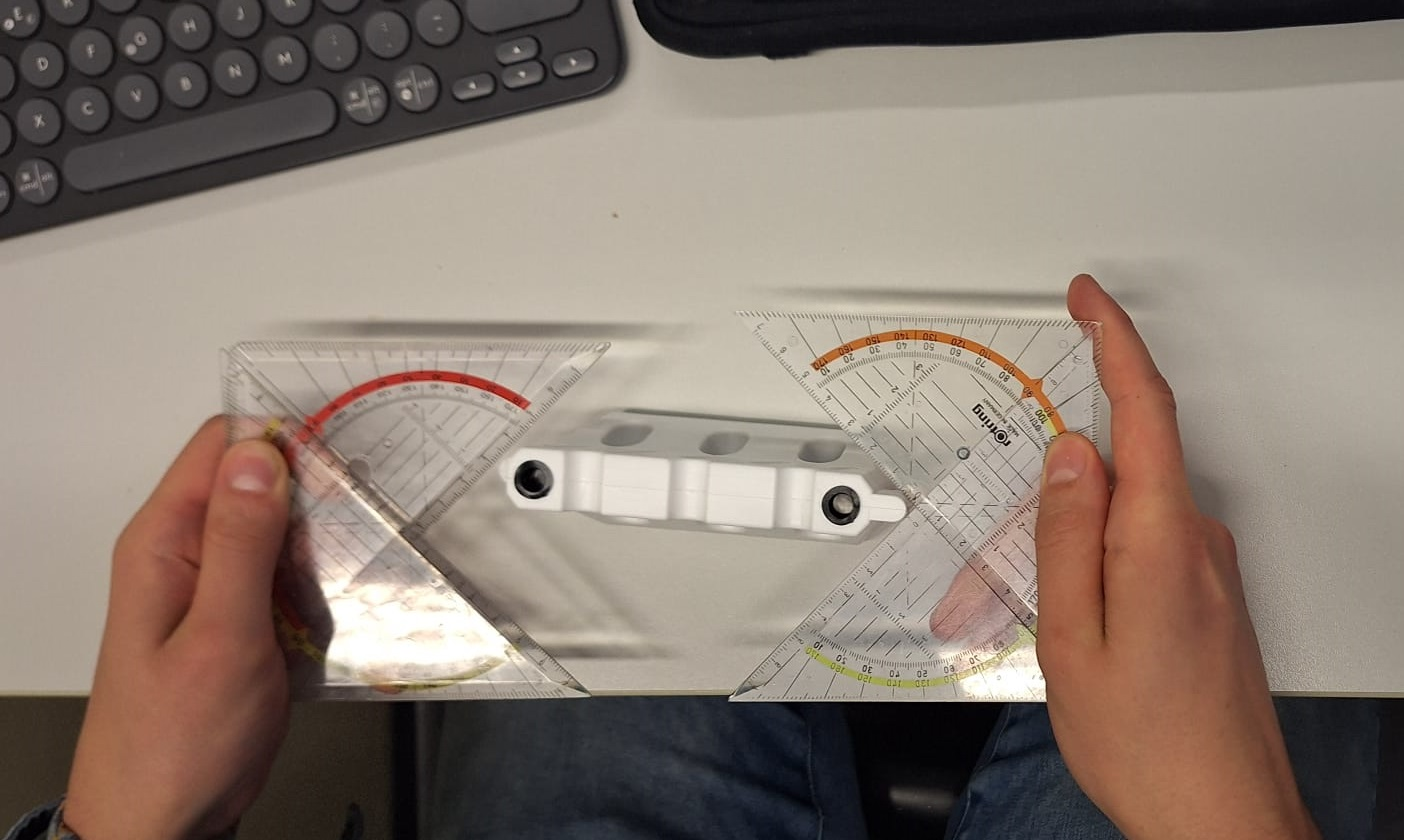
\includegraphics[width=\linewidth]{img/konzeptfindung/klemme_breitenweg_zentrierung_1.jpeg}
                    \caption{Darstellung Zentrierung bei Klemme seitlich - Bild 1}
                    \label{img:konzept_zentrierung_1}
                \end{minipage}
                \hfill
                \begin{minipage}{0.48\textwidth}
                    \centering
                    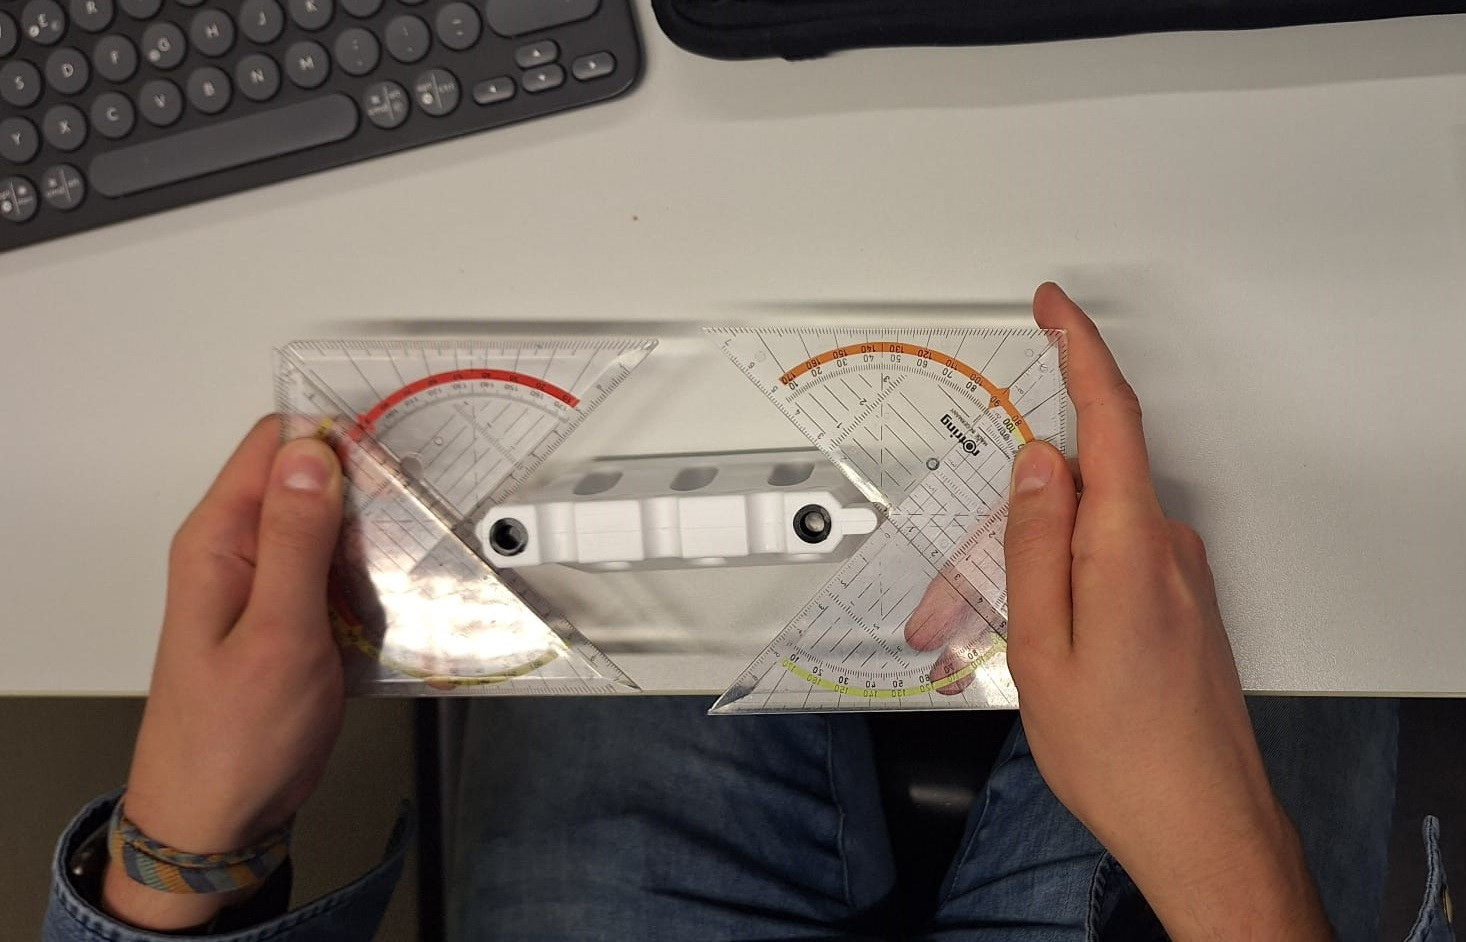
\includegraphics[width=\linewidth]{img/konzeptfindung/klemme_breitenweg_zentrierung_2.jpeg}
                    \caption{Darstellung Zentrierung bei Klemme seitlich - Bild 2}
                    \label{img:konzept_zentrierung_2}
                \end{minipage}
            \end{figure}


        \begin{figure}[h!]
            \centering
            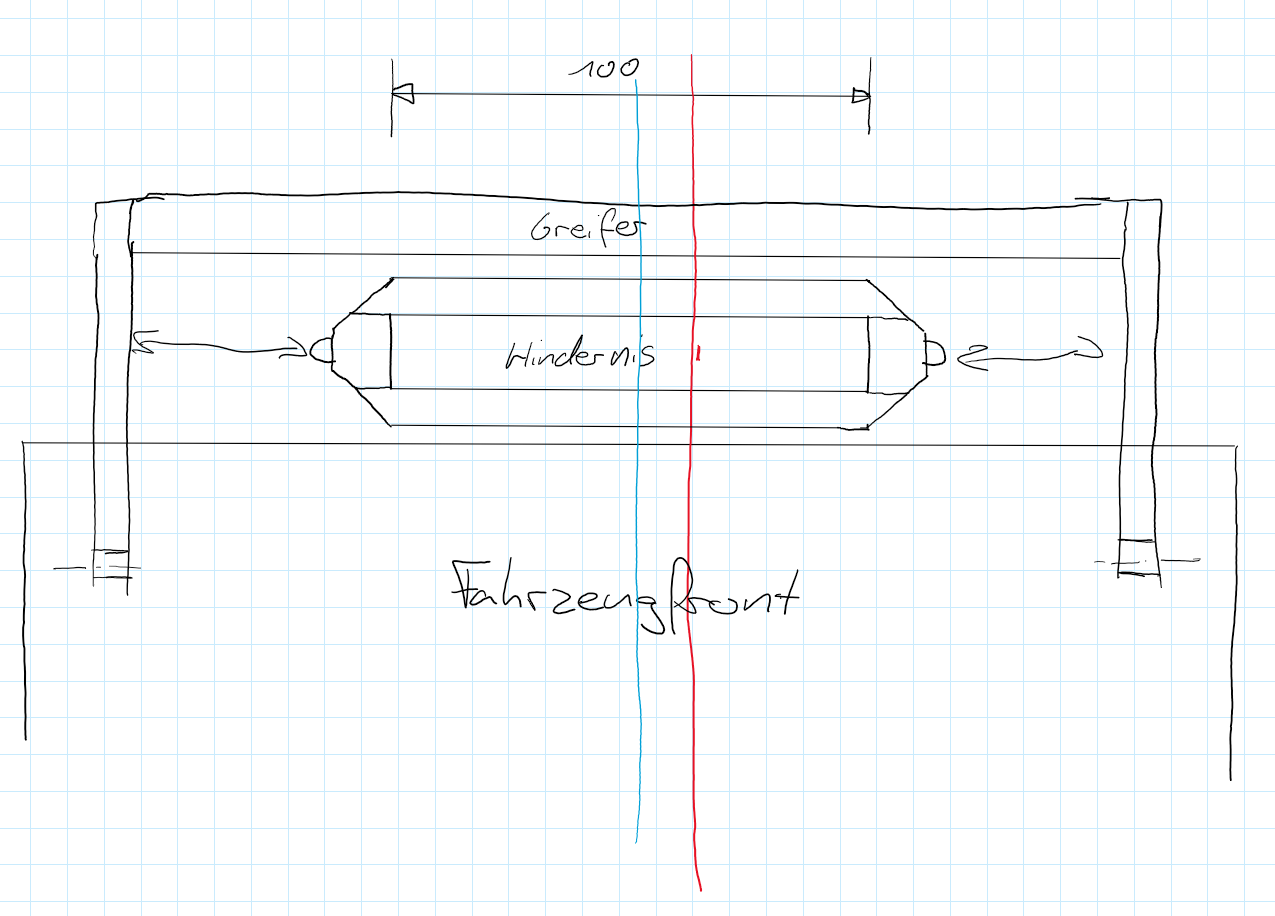
\includegraphics[width=0.48\textwidth]{img/konzeptfindung/Klemme_Langsweg_off_center.png}
            \caption{Darstellung 'Offset' bei Klemmung seitlich}
        \label{img:konzept_zentrierung_3}
        \end{figure}  

\newpage

\subsubsection{Konzept Aufnahme seitlich}
\label{a3:Aufnahme_seitlich}
Wie bereits beschrieben wurde das Greifkonzept 'Klemme seitlich' ausgewählt (siehe \ref{a3:Aufnahme_Hindernis}).
Damit dieses erfolgreich umgesetzt werden kann, wurden Dimensionen vom Greifer definiert  sowie ein passendes Konzept für den Mechanismus gefunden. Zusätzlich wurde der Hebemechanismus und der Greifmechanismus so konstruiert, dass es mit nur einem Motor angesteuert werden kann. Dies vereinfacht die Ansteuerung extrem und es werden weniger Sensoren benötigt.
Das Design, ersichtlich in Abbildung \ref{fig:greifarm_oben} und \ref{fig:greifarm_unten}, besteht aus einer Kombination von Zahnrädern für die Klemmen sowie einer linearen Bewegung für das Anheben der ganzen Konstruktion mit Hindernis.

\paragraph{Dimensionen Klemmmechanismus}
Wie bereits im Kapitel \ref{a3:Präzision} erwähnt, ist die Präzision, die mechanisch gewonnen werden kann, sehr relevant für dieses Konzept. Damit dies auch funktioniert, wurden die passenden Dimensionen der Klemme eruiert. 

\subparagraph{Winkel Verschiebung:} \label{loes:winkel_verschiebung}
Nach Aufgabenstellung kann das Hindernis bis zu 15° verschoben sein.
In der Abbildung \ref{img:loes_winkel_hinderniss} ist dies bildlich dargestellt.

\begin{figure}[H]
        \centering
        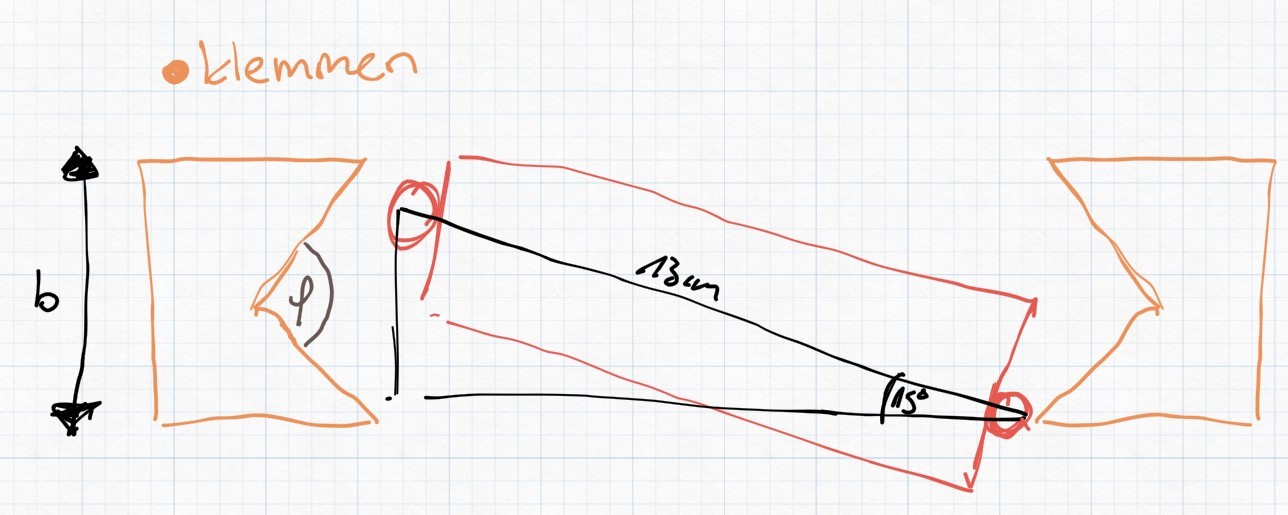
\includegraphics[width=0.48\textwidth]{img/lösungskonzpet/hindernissaufnahme/winkekl_klemmen.jpg}
        \caption {Möglicher Winkel des Hinderniss}
        \label{img:loes_winkel_hinderniss}
\end{figure}

Damit kann $b$ ausgerechnet werden:

\[
b = 13cm * sin(15) = 3.36cm
\]

Für genügend Sicherheit wurde entschieden das $b = 4.5cm$ ist. Diese Sicherheit hilft ebenfalls Fehler in der Distanzmessung auszugleichen.

$\varphi$ wurde als erste näherung 90° definiert. Die Winkeldefinition wurde anschliessend erfolgreich in Kapitel \ref{sec:hardware_greifarm} getestet.

\newpage

\subparagraph{Abstand der Klemmbacken:} \label{loes:abstand_klemmen}
Der Abstand der Klemmbacken wurde anhand der Aufgabenstellung eruiert und ist in Abbildung \ref{img:loes_abstand_klemmen} ersichtlich. Das Hindernis kann 2 cm von der Linie entfernt sein. Das heisst, das Maximale Offset ist 2 cm (in Abbildung Orange).(Hinweis: Diese Angabe zum Offset aus der Aufgabenstellung wurde erst nach dem Erstellen dieser Analyse reduziert) Zusätzlich kommt die Winkel Reserve, die Distanz wurde im Kapitel \ref{loes:winkel_verschiebung} eruiert (In der Abbildung Blau). Ebenfalls in der Abbildung enthalten sind Reserve für Fehlmessungen (Rot), Reserve Festigkeit, die für nötig ist, um die Druckkräfte auszuhalten (Violett) und die Hälfte des Hindernis (Gelb)

\begin{figure}[H]
        \centering
        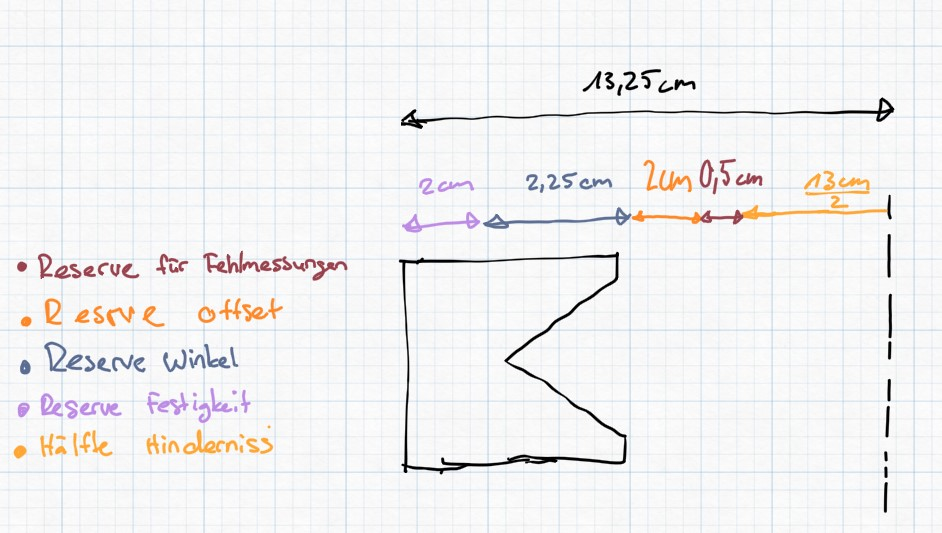
\includegraphics[width=0.48\textwidth]{img/lösungskonzpet/hindernissaufnahme/dimensionen_klemme.jpg}
        \caption {Abstand zwischen den Klemmbacken}
        \label{img:loes_abstand_klemmen}
\end{figure}

\newpage
\subsection{Morphologischer Kasten für Simulator} \label{sec:sim_Morphologischer_Kasten}

Dieser Abschnitt beschreibt die Erstellung eines Morphologischen Kastens für den Simulator. Der Morphologische Kasten ist in der Tabelle \ref{tab:sim_Morphologischer_Kasten} abgebildet. In den Unterkapiteln werden die Teilfunktionen im Morphologischen Kasten beschrieben und die gewählte Option begründet.  

Der Lösungsansatz des Morphologischen Kastens ist darauf ausgelegt, einen simplen Simulator zu erstellen, welcher trotzdem viele Anforderungen an die Wegfindung abdecken kann.

\newcolumntype{Y}{>{\centering\arraybackslash}X}

\begin{table}[htbp!]
    \centering
    \begin{tabularx}{\textwidth}{| X | Y | Y | Y |}
        \hline

        \rowcolor{LightGray}
        \textbf{Funktion} & \textbf{Option 1} & \textbf{Option 2} & \textbf{Option 3} \\ \hline
        
        \textbf{User Interface} &     
        Terminal \newline
        
\includegraphics[width=2.5cm]{img/simulation/morphologischer-kasten/terminal.png}
        &
        \cellcolor{LightGreen}
        Einfaches GUI \newline
        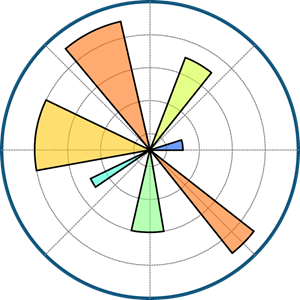
\includegraphics[width=2.5cm]{img/simulation/morphologischer-kasten/simple-gui.png}
        &
        Unreal Engine \newline
        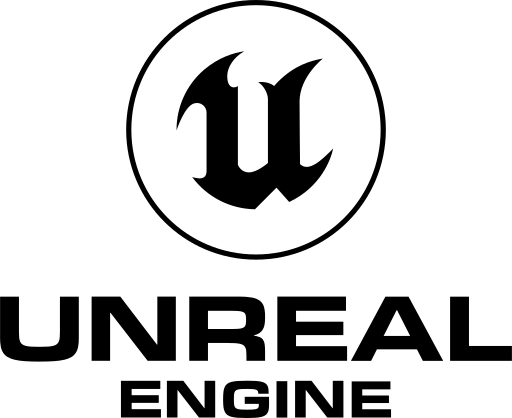
\includegraphics[width=2.5cm]{img/simulation/morphologischer-kasten/unreal-engine-logo.png}
        \\ \hline
        
        \textbf{Wegfindungs-Algorithmus}  &
        \cellcolor{LightGreen}
        Externe Bibliothek &
        Eigene Implementation &
        \\ \hline
        
        \textbf{Programmiersprache}      &
        \cellcolor{LightGreen}
        Python \newline
        
\includegraphics[width=2.5cm]{img/simulation/morphologischer-kasten/python.png} 
        &
        JavaScript \newline
        
\includegraphics[width=2.5cm]{img/simulation/morphologischer-kasten/javascript.png}
        &
        Java \newline
        
\includegraphics[width=2.5cm]{img/simulation/morphologischer-kasten/java.png}
        \\ \hline
        
        \textbf{Informationen \newline einlesen}  &     
        Bilder mit Objekterkennung \newline
        
\includegraphics[width=2.5cm]{img/simulation/morphologischer-kasten/ai-logo.jpg}
        &
        \cellcolor{LightGreen}
        Konfigurationsdatei \newline
        
\includegraphics[width=2.5cm]{img/simulation/morphologischer-kasten/yaml.png}
        &
        \\ \hline
        
        \textbf{Hindernis \newline Bewältigung}   &     
        Immer umfahren \newline
        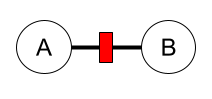
\includegraphics[width=3cm]{img/simulation/morphologischer-kasten/hindernis-umfahren.png}
        &
        Keine spezielle Behandlung \newline
        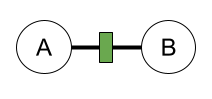
\includegraphics[width=3cm]{img/simulation/morphologischer-kasten/hindernis-ignoriert.png}
        &
        \cellcolor{LightGreen}
        Gewicht hinzufügen\newline
        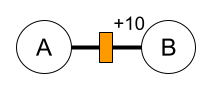
\includegraphics[width=3cm]{img/simulation/morphologischer-kasten/hindernis-gewicht.png}
        \\ \hline
    \end{tabularx}
    \caption{Morphologischer Kasten - Simulator}
    \label{tab:sim_Morphologischer_Kasten}
\end{table}

\subsubsection{User Interface}

Obwohl ebenfalls ein Digital Twin mit der Unreal Engine und dem Pfadfinder-Model existiert, ist der Aufwand zu gross, diese an den Simulator anzubinden. Eine Textbasierte Ausgabe auf einem Terminal hingegen ist zu minimal. Deshalb wird das User Interface mit einem einfachen GUI umgesetzt. 

\subsubsection{Wegfindungs-Algorithmus}

Die Umsetzung des Wegfindungs-Algorithmus kann entweder eigenständig oder mithilfe einer externen Bibliothek erfolgen. Da zahlreiche etablierte Bibliotheken für die Graphentheorie verfügbar sind, erscheint eine eigenständige Implementierung nicht sinnvoll. Dies führt zwar zu einer geringeren Flexibilität, reduziert jedoch die Fehleranfälligkeit erheblich.

\subsubsection{Programmiersprache}

Für die Wahl der Programmiersprache wurden Python, JavaScript und Java in Betracht gezogen. Java ist im Informatik-Studium weit verbreitet und wird für zahlreiche Projekte eingesetzt. JavaScript bietet die Möglichkeit, grafische Darstellungen unkompliziert über eine Webseite zu realisieren. Python zeichnet sich durch seine einfache Handhabung aus und wird häufig im Bereich der Künstlichen Intelligenz verwendet, was für die Software des autonomen Roboters wichtig ist.

Python wurde als Programmiersprache gewählt, da innerhalb des Teams umfassendes Know-how vorhanden ist. Darüber hinaus stellt die Bibliothek NetworkX\footnote{https://networkx.org} eine leistungsstarke Lösung für die Arbeit mit Graphen bereit, die optimal für die Anforderungen des Projekts geeignet ist.

\subsubsection{Informationen einlesen}

Damit die Software die Hindernisse auf dem Graphen kennt, müssen entsprechende Informationen eingelesen werden können. Idealerweise erfolgt dies ähnlich wie in der Realität, durch die Auswertung von Bildern mittels Objekterkennung. Um den Simulator jedoch möglichst schnell einsatzfähig zu machen, wird stattdessen eine Konfigurationsdatei verwendet, die die notwendigen Informationen bereitstellt.

Die Konfigurationsdatei ermöglicht eine einfache Anpassung der Szenarien und erlaubt dadurch das effiziente Testen verschiedener Konstellationen. Diese Herangehensweise beschleunigt die Entwicklungsphase und sorgt für Flexibilität beim Simulieren diverser Bedingungen.

\subsubsection{Hindernis Bewältigung}

Der Simulator soll aufzeigen, wie Hindernisse auf der Strecke behandelt werden.
Dabei wird berücksichtigt, dass Hindernisse unter bestimmten Bedingungen nicht immer umfahren werden können, beispielsweise wenn sämtliche alternativen Wege blockiert sind. Daher stellt die Option `Immer umfahren` keine sinnvolle Strategie dar.

Das Ignorieren von Hindernissen ist ebenfalls suboptimal, da gleich lange Pfade ohne Hindernisse effizienter befahren werden können. Um diesem Problem zu begegnen, wird die Strategie `Gewicht hinzufügen` angewendet. Mit dieser Methode kann flexibel entschieden werden, wie stark ein Hindernis die Wahl eines Pfades beeinflusst. Die Gewichtung erlaubt es, Hindernisse dynamisch in die Berechnung einzubeziehen, ohne zwingend alle Alternativen auszuschliessen.


\end{document}